\mySection{11.4 Covariance and Correlation}
%-------------- start slide -------------------------------%{{{ 11.9
\begin{frame}
	% {\S\: 11.4  Covariance and Correlation}
	\centering
	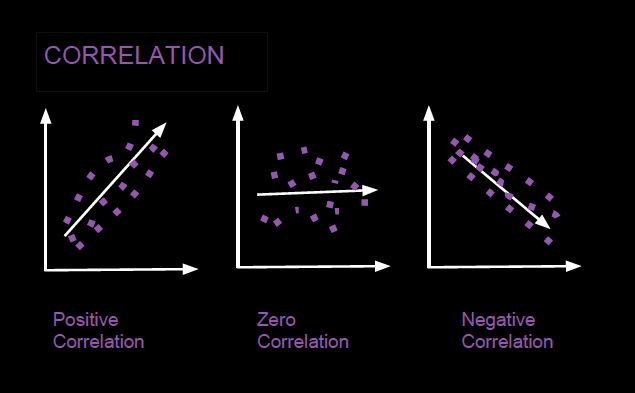
\includegraphics[scale=0.5]{Correlation_coefficent-neg.png}
\end{frame}
%-------------- end slide -------------------------------%}}}
%-------------- start slide -------------------------------%{{{ 11.10
\begin{frame}
	\centering
	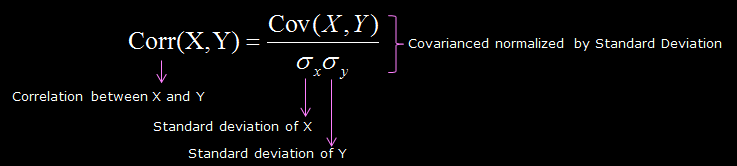
\includegraphics[scale=0.4]{Correlation_coefficent_Formula-neg.png}
\vfill

\begin{enumerate}
	\item[] Notation: $Corr(X,Y) = \rho(X,Y) = \rho_{XY}$\\[3em]
	\item[] Computing:  $\Var(X) = \sigma_X^2$, $\Var(Y)=\sigma_Y^2$, $\Cov(X,Y)=\sigma_{XY}$
	\item[]
		\[
			\Downarrow
		\]
		\[
			\rho_{XY} = \frac{\sigma_{XY}}{\sigma_X\sigma_Y}
		\]
\end{enumerate}
\end{frame}
%-------------- end slide -------------------------------%}}}
%-------------- start slide -------------------------------%{{{ 11.11
\begin{frame}

	\begin{enumerate}
		\item[Thm.] For any two random variables $X$ and $Y$,
		\item[a.] $|\rho(X,Y)| \le 1$
		\item[b.] $\rho(X,Y) = 1$ if and only if $Y=aX+b$ for some $a>0$ and $b\in\R$;
		\item[] $\rho(X,Y) = -1$ if and only if $Y=aX+b$ for some $a<0$ and $b\in\R$.
			\vfill
		\item[Proof.] (a)
			\begin{gather*}
				| \rho(X,Y) | \le 1 \\[1em]
				\Updownarrow
			\end{gather*}
			\begin{align*}
				\left| \E\left((X-\E(X))(Y-\E(Y))\right) \right| &\le \sqrt{\Var(X)\Var(Y)}\\
																												 &= \sqrt{\E\left((X-\E(X))^2\right)} \sqrt{\E\left((Y-\E(Y))^2\right)}
			\end{align*}
			which is nothing but the Cauchy-Schwartz inequality.
	\end{enumerate}
\end{frame}
%-------------- end slide -------------------------------%}}}
%-------------- start slide -------------------------------%{{{ 1
\begin{frame}[fragile]
\begin{itemize}
	\item[] (b) In the Cauchy-Schwartz inequality, the equality holds if and only if for some $a\ne 0$,
		\begin{align*}
			X-\E(X) = a [Y - E(Y)]
		\end{align*}
		namely,
		\begin{align*}
			X = a Y + b,\qquad \text{with}\quad b= \E(X) -a \E(Y).
		\end{align*}
	\item[] In particular, $a>0$ corresponds to the case $\rho(X,Y)=1$ and $a<0$ to $\rho(X,Y)=-1$.
		\myEnd
\end{itemize}
\end{frame}
%-------------- end slide -------------------------------%}}}l
%-------------- start slide -------------------------------%{{{ 11.12
\begin{frame}{Estimating $\rho(X,Y)$\\
	-- Sample correlation coefficient}

	\begin{enumerate}
		\item[]
	\begin{align*}
		\rho(X,Y) &=  \frac{\Cov(X,Y)}{\sqrt{\Var(X)}\sqrt{\Var(Y)}}\\[2em]
& =  \frac{\E[X Y] -\E[X]\E[Y]}{\sqrt{\E[X^2]-\E[X]^2}\sqrt{\E[Y^2]-\E[Y]^2}}
	\end{align*}
	\vfill
\item[] \[\Downarrow\]
	\vfill
\item[]
	\[
		R =  \frac{n\sum_{i=1}^n X_iY_i -\left(\sum_{i=1}^n X_i \right )\left(\sum_{i=1}^n Y_i \right ) }{\sqrt{n\sum_{i=1}^n X_i^2- \left(\sum_{i=1}^n X_i \right )^2}\sqrt{n\sum_{i=1}^n Y_i^2- \left(\sum_{i=1}^n Y_i \right )^2}}
	\]
	\vfill
\item[]
	\begin{center}
		{\it \textcolor{yellow}{Pearson product-moment correlation coefficient}}\\[1em]
	or \\[1em]
	{\it \textcolor{yellow}{Sample correlation coefficient}}
	\end{center}
	\end{enumerate}
\end{frame}
%-------------- end slide -------------------------------%}}}
%-------------- start slide -------------------------------%{{{ 11.13
\begin{frame}

	\begin{enumerate}
		\item[Thm.] $$R^2 = 1 - \frac{SSE}{SST} = \frac{SST-SSE}{SST} = \frac{SSTR}{SST} $$ where
			\[
				SSE = \sum_{i=1}^n \left(Y_i - \widehat{Y}_i \right)^2, \quad \widehat{Y_i} = \hat{\beta}_0+\hat{\beta}_1 X_i
			\]
			\[
				SST =  \sum_{i=1}^n \left(Y_i - \overline{Y}_i \right)^2, \quad\text{and}\quad
				SSTR = SST-SSE.
			\]
			\vfill
		\item[Remark] SSE: sum of square errors $\sim$ the variation in $y_i$'s not explained by L.M.\\[1em]
		\item[] SST: Total sum of squares $\sim$ total variability. \\[1em]
		\item[] SSTR: Treatment sum of sqrs. $\sim$ the variation in $y_i$'s explained by L.M. \\[1em]
		\item[] $R^2$ (or $r^2$ when $X_i$ and $Y_i$ are replaced by $x_i$ and $y_i$) $\sim$ proportion of total variation in the $y_i$'s that can be attributed to L.M.  \\
		\item[]
			\begin{center}
			{\it Coefficient of determination} or simply {\it R squared}
			\end{center}
	\end{enumerate}
\end{frame}
%-------------- end slide -------------------------------%}}}
%-------------- start slide -------------------------------%{{{ 11.14
\begin{frame}
	\OneFrame{Proof}
\end{frame}
%-------------- end slide -------------------------------%}}}
%-------------- start slide -------------------------------%{{{ 11.15
\begin{frame}{Adjusted R-squared}

	\begin{enumerate}
		\item[Def.] The adjusted R-squareed:
	\[
		R^2_{adj} := 1-\frac{MSE}{MST}
	\]
where
\[
	MSE = \frac{SSE}{n-q} \qquad\text{and}\qquad MST = \frac{SST}{n-1}
\]
and $q$ is number of parameters in the model.
\vfill
\item[Relation:]
	\[
		R^2_{adj} = 1- \left(1-R^2\right) \frac{n-1}{n-q}
	\]
	\vfill
\item[] MSE: Mean squared error.
\item[] MST: Mean squared total.
\item[] MSR = MSTR: Mean square for treatment (or regresssion).
	\[
		MSR = MSTR = \frac{SSTR}{q-1}
	\]
	\end{enumerate}
\end{frame}
%-------------- end slide -------------------------------%}}}
